%!TEX root = ../main.tex



\section{sommario}

\begin{itemize}
    \item \textbf{Pose of a Rigid Body} (slides 3--7)
    \begin{itemize}
        \item Position and orientation of a rigid body (3)
        \item Reference frame and body-attached frame (4--5)
        \item Orientation as unit vectors of frame 1 expressed in frame 0 (6)
        \item Planar case (7)
    \end{itemize}

    \item \textbf{Rotation Matrix} (slides 8--16)
    \begin{itemize}
        \item Definition, orthonormality of columns, group $SO(m)$ (8--10)
        \item Elementary rotation matrices (11--12)
        \item Rotation matrix as a coordinate transformation (13--14)
        \item Rotation matrix as an operator (15)
        \item Composition of rotation matrices (16)
    \end{itemize}

    \item \textbf{Other Representations of Orientation} (slides 17--35)
    \begin{itemize}
        \item Redundancy of rotation matrices and minimal representations (17)
        \item Euler angles, ZYZ sequence and inverse problem (18--21)
        \item Roll--Pitch--Yaw angles, XYZ sequence and inverse problem (22--24)
        \item Axis--angle representation and inverse problem (25--28)
        \item Unit quaternion, inverse and composition (29--32)
        \item Exponential coordinates, skew-symmetric matrix (33--35)
    \end{itemize}

    \item \textbf{Homogeneous Transformations} (slides 36--40)
    \begin{itemize}
        \item Combining translation and rotation in one operator (36--38)
        \item Homogeneous coordinates and $4\times4$ transformation matrix (39)
        \item Inverse homogeneous transformation (40)
    \end{itemize}

    \item \textbf{Configuration Space} (slides 41--51)
    \begin{itemize}
        \item Robot as a set of rigid bodies connected by joints (revolute, prismatic), end-effector (41--43)
        \item Generalized coordinates, configuration and configuration space $\mathcal{C}$ (44--46)
        \item Example: 2R planar arm and topology of its configuration space (47--48)
        \item Distance in configuration space, control points (49--51)
    \end{itemize}

    \item \textbf{Task Space and Direct Kinematics} (slides 52--55)
    \begin{itemize}
        \item Tasks, task coordinates and task space (52--53)
        \item Kinematic redundancy and degree of redundancy (54--55)
    \end{itemize}

    \item \textbf{Direct Kinematics of Manipulators} (slides 56--78)
    \begin{itemize}
        \item Direct kinematics map $y = k(q)$ and end-effector tasks (56--61)
        \item Open-chain manipulators, composition of transformations (62--64)
        \item Denavit--Hartenberg convention: frame assignment, parameters, transformation, procedure (65--71)
        \item Extension to closed-chain manipulators: loop closure constraints, cut joint, procedure (72--78)
    \end{itemize}

    \item \textbf{Examples of Direct Kinematics} (slides 79--106)
    \begin{itemize}
        \item 3R planar arm (80--83)
        \item Parallelogram arm (84--88)
        \item SCARA manipulator (89--92)
        \item Anthropomorphic arm (93--96)
        \item Spherical wrist (97--100)
        \item 6R manipulator with spherical wrist (101--103)
        \item DLR manipulator (7 DoF, redundant) (104--106)
    \end{itemize}

    \item \textbf{Kinematic Calibration} (slides 107--116)
    \begin{itemize}
        \item Calibration problem: deviations of actual from nominal DH parameters (107--108)
        \item First-order linearization and stacked measurements (109--111)
        \item Least-squares solution with pseudoinverse (112)
        \item Iterative algorithm for the nonlinear problem (113--115)
        \item Repeatability (116)
    \end{itemize}

    \item \textbf{Reachable Workspace} (slides 117--120)
    \begin{itemize}
        \item Definition of reachable workspace $W_r$ (117)
        \item Dependence on geometry and joint limits (118)
        \item Example: 2R planar arm, elbow-up / elbow-down (119)
        \item Representation in manufacturer data sheets (120)
    \end{itemize}

    \item \textbf{Inverse Kinematics} (slides 121--136)
    \begin{itemize}
        \item Problem statement and closed-form solutions (121--122)
        \item 3R planar arm, wrist center, admissible postures (123--127)
        \item Manipulators with spherical wrist, decoupling of position and orientation (128--129)
        \item Inverse kinematics of the spherical wrist (130--131)
        \item Inverse kinematics of the anthropomorphic arm, admissible postures (132--136)
    \end{itemize}
\end{itemize}

\pagebreak

\section{Foundations of Robotics: Kinematics}

%==================================================
\subsection{Kinematics}
%==================================================



\begin{defbox}{Kinematics}
Kinematics is the study of the \textbf{motion of bodies without considering the causes} that produce it (forces and torques). It only deals with geometry: positions, orientations and, later, velocities.
\end{defbox}

In robotics, kinematics answers the question: \emph{given the values of the joints of a robot, where is its end-effector (gripper/tool) and how is it oriented, and vice versa?} The study of forces and torques belongs to \emph{dynamics}, which is a separate topic.

%==================================================

%==================================================

\subsubsection{Outline}

 The roadmap of the whole chapter is:

\begin{itemize}
    \item Pose of a Rigid Body
    \item Rotation Matrix
    \item Other Representations of Orientation
    \item Homogeneous Transformations
    \item Configuration Space
    \item Task Space and Direct Kinematics
    \item Direct Kinematics of Manipulators
    \item Examples of Direct Kinematics
    \item Kinematic Calibration
    \item Reachable Workspace
    \item Inverse Kinematics
\end{itemize}

\paragraph{Logic of the roadmap.} The order is bottom-up:
\begin{enumerate}
    \item first we learn how to describe \emph{one} rigid body in space (pose, rotation matrices, other orientation representations, homogeneous transformations);
    \item then we describe a \emph{robot} as a chain of rigid bodies connected by joints (configuration space, task space);
    \item finally we relate the two descriptions: \textbf{direct kinematics} (from joints to end-effector pose) and \textbf{inverse kinematics} (from end-effector pose to joints). Calibration and workspace are practical issues on top of these.
\end{enumerate}

\begin{center}
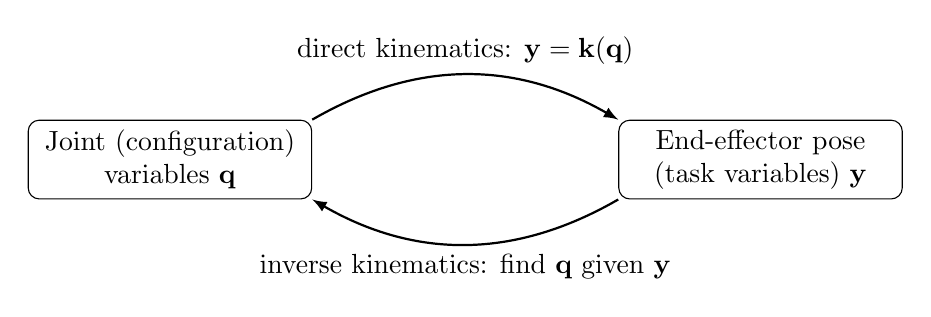
\begin{tikzpicture}[>=latex, box/.style={draw, rounded corners, minimum height=1cm, minimum width=3.6cm, align=center}]
  \node[box] (q) at (0,0) {Joint (configuration)\\ variables $\mathbf{q}$};
  \node[box] (y) at (7.5,0) {End-effector pose\\ (task variables) $\mathbf{y}$};
  \draw[->, thick] (q.north east) to[bend left] node[above] {direct kinematics: $\mathbf{y}=\mathbf{k}(\mathbf{q})$} (y.north west);
  \draw[->, thick] (y.south west) to[bend left] node[below] {inverse kinematics: find $\mathbf{q}$ given $\mathbf{y}$} (q.south east);
\end{tikzpicture}
\end{center}

The variables $\mathbf{q}$ and $\mathbf{y}$ are formally introduced later in the chapter; the scheme is only a preview of where we are heading.

%==================================================
\subsubsection{Pose of a Rigid Body}
%==================================================

\begin{defbox}{Rigid body}
A rigid body is an idealized body that \textbf{does not deform}: the distance between any two of its points stays constant during any motion.
\end{defbox}

Since the body is rigid, describing \emph{where the whole body is} reduces to describing where \emph{one} of its points and its ``direction in space'' are. This gives two ingredients:
\begin{itemize}
    \item \textbf{position}: where the body is located (3 numbers in space);
    \item \textbf{orientation}: how the body is rotated with respect to a reference (3 independent numbers in space, as will be shown later).
\end{itemize}

\begin{defbox}{Pose}
The \textbf{pose} of a rigid body is the pair (position, orientation). A free rigid body in space has therefore $3+3=6$ degrees of freedom (DoF).
\end{defbox}

\begin{center}
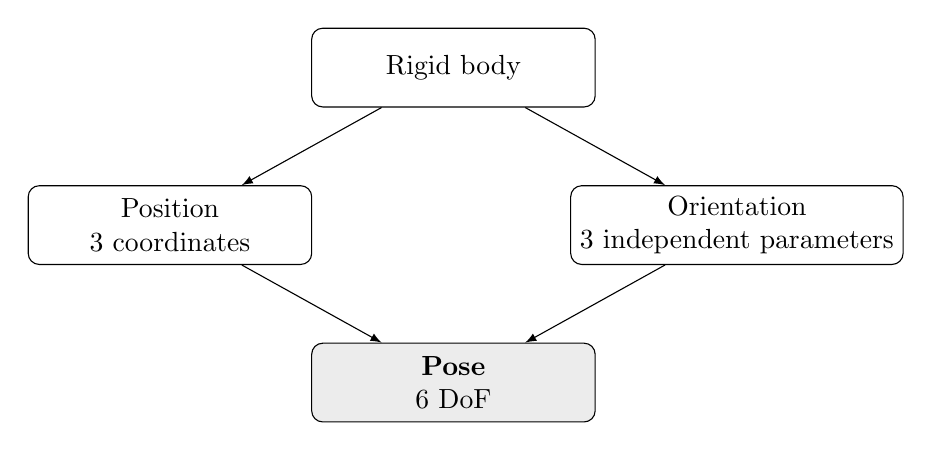
\begin{tikzpicture}[>=latex, box/.style={draw, rounded corners, align=center, minimum height=1cm, minimum width=3.6cm}]
  \node[box] (rb) at (0,0) {Rigid body};
  \node[box] (pos) at (-3.6,-2) {Position\\ 3 coordinates};
  \node[box] (ori) at (3.6,-2) {Orientation\\ 3 independent parameters};
  \node[box, fill=gray!15] (pose) at (0,-4) {\textbf{Pose}\\ 6 DoF};
  \draw[->] (rb) -- (pos);
  \draw[->] (rb) -- (ori);
  \draw[->] (pos) -- (pose);
  \draw[->] (ori) -- (pose);
\end{tikzpicture}
\end{center}

\paragraph{Reference frame attached to the body.} To give numbers to position and orientation, we attach a \textbf{reference frame} to the body: an origin $O$ (a point of the body) and three axes $x,y,z$ fixed to the body. The frame moves together with the body, so \emph{the pose of the frame is the pose of the body}.

\begin{defbox}{Orthogonal right-handed frame $O$--$xyz$}
A frame $O$--$xyz$ is described by three unit vectors $\mathbf{x},\mathbf{y},\mathbf{z}$ along its axes such that:
\begin{itemize}
    \item \textbf{unit norm}: $\mathbf{x}^T\mathbf{x}=\mathbf{y}^T\mathbf{y}=\mathbf{z}^T\mathbf{z}=1$;
    \item \textbf{orthogonality}: $\mathbf{x}^T\mathbf{y}=\mathbf{x}^T\mathbf{z}=\mathbf{y}^T\mathbf{z}=0$;
    \item \textbf{right-handedness}: $\mathbf{z}=\mathbf{x}\times\mathbf{y}$ (equivalently $\mathbf{x}=\mathbf{y}\times\mathbf{z}$, $\mathbf{y}=\mathbf{z}\times\mathbf{x}$). With the right hand, thumb $=\mathbf{x}$, index $=\mathbf{y}$, middle finger $=\mathbf{z}$.
\end{itemize}
\end{defbox}

\paragraph{Math recap.} For two vectors $\mathbf{a},\mathbf{b}$, the scalar product is $\mathbf{a}^T\mathbf{b}=\|\mathbf{a}\|\,\|\mathbf{b}\|\cos\theta$, where $\theta$ is the angle between them. It is zero when the vectors are orthogonal, and equal to $\cos\theta$ when both are unit vectors. This fact is the key to the next slides.

\paragraph{Notation.} When several frames are present, an \textbf{index (subscript)} is added to the frame and to its axes: frame $O_0$--$x_0y_0z_0$ has unit vectors $\mathbf{x}_0,\mathbf{y}_0,\mathbf{z}_0$, frame $O_1$--$x_1y_1z_1$ has unit vectors $\mathbf{x}_1,\mathbf{y}_1,\mathbf{z}_1$, and so on.

%==================================================
\subsubsection{Reference frame and body frame}
%==================================================

Two frames are used to describe the pose of the body:
\begin{itemize}
    \item $O_0$--$x_0y_0z_0$: the \textbf{reference frame} (fixed, e.g.\ the base of the robot or the ``world'');
    \item $O_1$--$x_1y_1z_1$: the frame \textbf{attached to the rigid body}, which moves with it.
\end{itemize}

\begin{center}
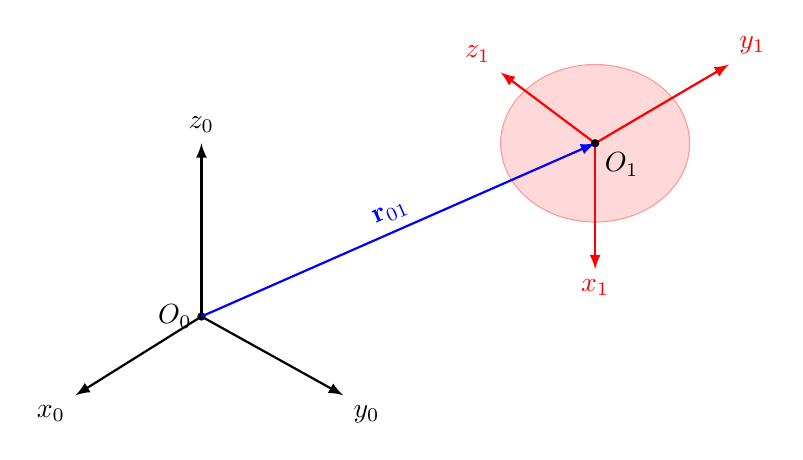
\begin{tikzpicture}[>=latex]
  % reference frame
  \draw[->, thick] (0,0) -- (0,2.2) node[above] {$z_0$};
  \draw[->, thick] (0,0) -- (-1.6,-1.0) node[below left] {$x_0$};
  \draw[->, thick] (0,0) -- (1.8,-1.0) node[below right] {$y_0$};
  \fill (0,0) circle (1.5pt) node[left] {$O_0$};
  % rigid body
  \draw[fill=red!15, draw=red!40] (5,2.2) ellipse (1.2 and 1.0);
  % body frame
  \draw[->, thick, red] (5,2.2) -- (5,0.6) node[below] {$x_1$};
  \draw[->, thick, red] (5,2.2) -- (6.7,3.2) node[above right] {$y_1$};
  \draw[->, thick, red] (5,2.2) -- (3.8,3.1) node[above left] {$z_1$};
  \fill (5,2.2) circle (1.5pt) node[below right] {$O_1$};
  % position vector
  \draw[->, thick, blue] (0,0) -- (5,2.2) node[midway, above, sloped] {$\mathbf{r}_{01}$};
\end{tikzpicture}
\end{center}

The blue arrow $\mathbf{r}_{01}$ (position of $O_1$ w.r.t.\ $O_0$) and the orientation of the red axes w.r.t.\ the black axes contain everything we need: this is exactly what the next chapter formalize.

The choice of which frame is ``reference'' and which is ``attached'' is a convention. In manipulators, frame 0 will typically be attached to the fixed base and the last frame to the end-effector.

%==================================================
\subsubsection{Position of the body}
%==================================================

The pose of the rigid body is described by
\begin{itemize}
    \item the \textbf{position} of $O_1$ with respect to $O_0$;
    \item the \textbf{orientation} of frame $O_1$--$x_1y_1z_1$ with respect to $O_0$--$x_0y_0z_0$.
\end{itemize}

\begin{defbox}{Position vector}
The position of $O_1$ with respect to $O_0$ is the vector $\mathbf{r}_{01}\in\mathbb{R}^3$, going from $O_0$ to $O_1$. Expressed in frame 0 it is
\[
{}^{0}\mathbf{r}_{01}={}^{0}r_x\,\mathbf{x}_0+{}^{0}r_y\,\mathbf{y}_0+{}^{0}r_z\,\mathbf{z}_0=
\begin{bmatrix}{}^{0}r_x\\ {}^{0}r_y\\ {}^{0}r_z\end{bmatrix}.
\]
\end{defbox}

\paragraph{Understanding the notation.}
\begin{itemize}
    \item The \textbf{left superscript} (here $0$) tells in which frame the vector is \emph{expressed}, i.e.\ with respect to which axes the coordinates are computed.
    \item The \textbf{subscript} $01$ tells that the vector goes from $O_0$ to $O_1$.
    \item ${}^0r_x,{}^0r_y,{}^0r_z$ are the coordinates of $\mathbf{r}_{01}$ along $\mathbf{x}_0,\mathbf{y}_0,\mathbf{z}_0$. Since the axes are orthonormal, each coordinate is the \textbf{projection} of the vector on the corresponding axis: ${}^0r_x=\mathbf{x}_0^T\,\mathbf{r}_{01}$, and similarly for $y$ and $z$.
\end{itemize}

The geometric vector $\mathbf{r}_{01}$ is a physical object that does not depend on the frame; its \emph{coordinates} do. The same vector written in another frame would have a different column of numbers, which is why the superscript is essential.

\begin{example}
Suppose $O_1$ is located $2$ m along $\mathbf{x}_0$, $1$ m along $\mathbf{y}_0$ and $3$ m along $\mathbf{z}_0$ from $O_0$.
\begin{itemize}
    \item \texttt{Step 1: Identify the two frames.} $O_0$ is the reference, $O_1$ is the point whose position we want.
    \vspace{0.2cm}
    \item \texttt{Step 2: Write the vector as a combination of the axes.} ${}^0\mathbf{r}_{01}=2\,\mathbf{x}_0+1\,\mathbf{y}_0+3\,\mathbf{z}_0$.
    \vspace{0.2cm}
    \item \texttt{Step 3: Collect the coordinates.} ${}^0\mathbf{r}_{01}=\begin{bmatrix}2&1&3\end{bmatrix}^T$, and its length is $\|\mathbf{r}_{01}\|=\sqrt{2^2+1^2+3^2}=\sqrt{14}\approx 3.74$ m.
\end{itemize}
\end{example}

%==================================================
\subsubsection{Orientation of the body}
\label{Orientation of the body}
%==================================================

Orientation is described by the \textbf{unit vectors of frame 1 expressed in frame 0}. Each of the three axes of the body frame is written as a combination of the axes of the reference frame:
\begin{align*}
{}^0\mathbf{x}_1 &= {}^0x_x\,\mathbf{x}_0+{}^0x_y\,\mathbf{y}_0+{}^0x_z\,\mathbf{z}_0,\\
{}^0\mathbf{y}_1 &= {}^0y_x\,\mathbf{x}_0+{}^0y_y\,\mathbf{y}_0+{}^0y_z\,\mathbf{z}_0,\\
{}^0\mathbf{z}_1 &= {}^0z_x\,\mathbf{x}_0+{}^0z_y\,\mathbf{y}_0+{}^0z_z\,\mathbf{z}_0.
\end{align*}

\paragraph{Notation.} ${}^0y_x$ means: the $x$-component (along $\mathbf{x}_0$) of the vector $\mathbf{y}_1$, expressed in frame 0. The letter is the vector, the subscript is the component.

\begin{defbox}{Direction cosines}
The nine coordinates above are the \textbf{direction cosines} of the axes of frame $O_1$--$x_1y_1z_1$ with respect to frame $O_0$--$x_0y_0z_0$. Each one is a scalar product of two unit vectors, for example
\[
{}^0y_x=\mathbf{x}_0^T\,\mathbf{y}_1=\|\mathbf{x}_0\|\,\|\mathbf{y}_1\|\cos\theta=\cos\theta ,
\]
where $\theta$ is the angle between $\mathbf{x}_0$ and $\mathbf{y}_1$.
\end{defbox}

\paragraph{Why ``cosines''?} Because both vectors have norm 1, the scalar product reduces to the cosine of the angle between them. If two axes are parallel the value is $1$, if they are orthogonal it is $0$, if they are opposite it is $-1$.

\begin{center}
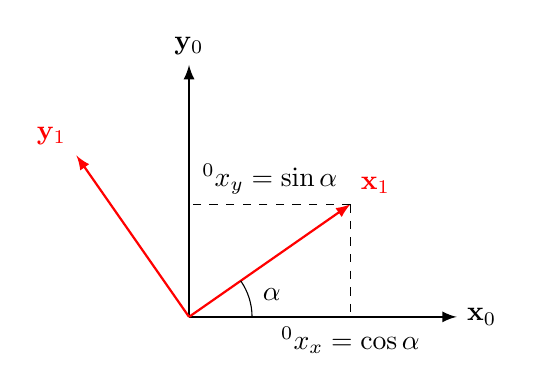
\begin{tikzpicture}[>=latex]
  \draw[->, thick] (0,0) -- (3.4,0) node[right] {$\mathbf{x}_0$};
  \draw[->, thick] (0,0) -- (0,3.2) node[above] {$\mathbf{y}_0$};
  \draw[->, thick, red] (0,0) -- (2.05,1.43) node[above right] {$\mathbf{x}_1$};
  \draw[->, thick, red] (0,0) -- (-1.43,2.05) node[above left] {$\mathbf{y}_1$};
  \draw[dashed] (2.05,1.43) -- (2.05,0) node[below] {${}^0x_x=\cos\alpha$};
  \draw[dashed] (2.05,1.43) -- (0,1.43) node[midway, above] {${}^0x_y=\sin\alpha$};
  \draw (0.8,0) arc (0:35:0.8);
  \node at (1.05,0.28) {$\alpha$};
\end{tikzpicture}
\end{center}

The figure shows the idea in 2D: the direction cosines of $\mathbf{x}_1$ are simply its projections on the axes of frame 0.

\paragraph{Theory integration: constraints.} The nine numbers are not independent. Since the axes of frame 1 are orthonormal, each triple has unit norm (3 conditions, e.g.\ $({}^0x_x)^2+({}^0x_y)^2+({}^0x_z)^2=1$) and the three vectors are mutually orthogonal (3 conditions). That gives $9-6=3$ independent parameters, consistent with the 3 degrees of freedom of orientation. In the next slides these nine numbers will be collected as the columns of the \textbf{rotation matrix}.

\begin{example}
Frame 1 is obtained from frame 0 by a rotation of $90^\circ$ about $\mathbf{z}_0$, so that $\mathbf{x}_1=\mathbf{y}_0$, $\mathbf{y}_1=-\mathbf{x}_0$, $\mathbf{z}_1=\mathbf{z}_0$. Find the direction cosines.
\begin{itemize}
    \item \texttt{Step 1: Compute the components of} $\mathbf{x}_1$. ${}^0x_x=\mathbf{x}_0^T\mathbf{y}_0=0$, \; ${}^0x_y=\mathbf{y}_0^T\mathbf{y}_0=1$, \; ${}^0x_z=\mathbf{z}_0^T\mathbf{y}_0=0$.
    \vspace{0.2cm}
    \item \texttt{Step 2: Compute the components of} $\mathbf{y}_1$. ${}^0y_x=\mathbf{x}_0^T(-\mathbf{x}_0)=-1$, \; ${}^0y_y=0$, \; ${}^0y_z=0$.
    \vspace{0.2cm}
    \item \texttt{Step 3: Compute the components of} $\mathbf{z}_1$. ${}^0z_x=0$, \; ${}^0z_y=0$, \; ${}^0z_z=1$.
    \vspace{0.2cm}
    \item \texttt{Step 4: Write the result.} 
    \[
    {}^0\mathbf{x}_1=\begin{bmatrix}0\\1\\0\end{bmatrix},\quad
    {}^0\mathbf{y}_1=\begin{bmatrix}-1\\0\\0\end{bmatrix},\quad
    {}^0\mathbf{z}_1=\begin{bmatrix}0\\0\\1\end{bmatrix}.
    \]
    \vspace{0.2cm}
    \item \texttt{Step 5: Sanity check.} Each vector has unit norm, they are mutually orthogonal, and $\mathbf{x}_1\times\mathbf{y}_1=\mathbf{y}_0\times(-\mathbf{x}_0)=\mathbf{x}_0\times\mathbf{y}_0=\mathbf{z}_0=\mathbf{z}_1$, so the frame is right-handed.
\end{itemize}
\end{example}

%==================================================
\subsubsection{The planar case}
%==================================================

In many problems (mobile robots on the floor, planar arms) the body moves in a plane, here the $x_0y_0$ plane. Each frame is then described by $O$--$xy$ and two unit vectors $\mathbf{x},\mathbf{y}$ (the axis $z$, orthogonal to the plane, stays common to both frames and carries no information).

\begin{defbox}{Planar pose}
In the plane, position and orientation reduce to the 2D case:
\[
{}^0\mathbf{r}_{01}={}^0r_x\,\mathbf{x}_0+{}^0r_y\,\mathbf{y}_0=\begin{bmatrix}{}^0r_x\\ {}^0r_y\end{bmatrix},
\qquad
\begin{aligned}
{}^0\mathbf{x}_1&={}^0x_x\,\mathbf{x}_0+{}^0x_y\,\mathbf{y}_0,\\
{}^0\mathbf{y}_1&={}^0y_x\,\mathbf{x}_0+{}^0y_y\,\mathbf{y}_0.
\end{aligned}
\]
\end{defbox}

\paragraph{Theory integration: only three parameters.} Position has 2 coordinates. For orientation there are 4 direction cosines, but unit norm and orthogonality impose 3 constraints, leaving \textbf{one} free parameter: the rotation angle $\alpha$ between $\mathbf{x}_0$ and $\mathbf{x}_1$. Using the cosine interpretation of \ref{Orientation of the body},
\begin{align*}
{}^0\mathbf{x}_1 &= \cos\alpha\,\mathbf{x}_0+\sin\alpha\,\mathbf{y}_0,\\
{}^0\mathbf{y}_1 &= -\sin\alpha\,\mathbf{x}_0+\cos\alpha\,\mathbf{y}_0.
\end{align*}
Hence a planar rigid body has $2+1=3$ DoF, versus $6$ in space.

\begin{center}
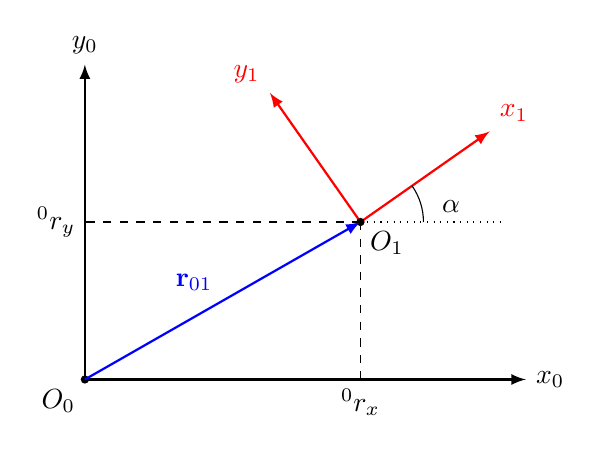
\begin{tikzpicture}[>=latex]
  % frame 0
  \draw[->, thick] (0,0) -- (5.6,0) node[right] {$x_0$};
  \draw[->, thick] (0,0) -- (0,4) node[above] {$y_0$};
  \fill (0,0) circle (1.5pt) node[below left] {$O_0$};
  % frame 1 (rotated by alpha = 35 degrees)
  \draw[->, thick, red] (3.5,2) -- (5.14,3.15) node[above right] {$x_1$};
  \draw[->, thick, red] (3.5,2) -- (2.35,3.64) node[above left] {$y_1$};
  \fill (3.5,2) circle (1.5pt) node[below right] {$O_1$};
  % position vector and its components
  \draw[->, thick, blue] (0,0) -- (3.5,2) node[midway, above left] {$\mathbf{r}_{01}$};
  \draw[dashed] (3.5,2) -- (3.5,0) node[below] {${}^0r_x$};
  \draw[dashed] (3.5,2) -- (0,2) node[left] {${}^0r_y$};
  % angle alpha
  \draw[dotted] (3.5,2) -- (5.3,2);
  \draw (4.3,2) arc (0:35:0.8);
  \node at (4.65,2.2) {$\alpha$};
\end{tikzpicture}
\end{center}

\begin{example}
A planar body has its frame origin at ${}^0\mathbf{r}_{01}=[3\;\;2]^T$ m and is rotated by $\alpha=30^\circ$ with respect to frame 0. Describe its pose.
\begin{itemize}
    \item \texttt{Step 1: Position.} ${}^0r_x=3$ m, ${}^0r_y=2$ m.
    \vspace{0.2cm}
    \item \texttt{Step 2: Direction cosines of} $\mathbf{x}_1$. ${}^0\mathbf{x}_1=\begin{bmatrix}\cos30^\circ\\ \sin30^\circ\end{bmatrix}=\begin{bmatrix}\sqrt3/2\\ 1/2\end{bmatrix}\approx\begin{bmatrix}0.866\\0.5\end{bmatrix}$.
    \vspace{0.2cm}
    \item \texttt{Step 3: Direction cosines of} $\mathbf{y}_1$. ${}^0\mathbf{y}_1=\begin{bmatrix}-\sin30^\circ\\ \cos30^\circ\end{bmatrix}\approx\begin{bmatrix}-0.5\\0.866\end{bmatrix}$.
    \vspace{0.2cm}
    \item \texttt{Step 4: Check.} $\|{}^0\mathbf{x}_1\|=\sqrt{0.866^2+0.5^2}=1$ and ${}^0\mathbf{x}_1^T\,{}^0\mathbf{y}_1=-0.866\cdot0.5+0.5\cdot0.866=0$, as required for an orthonormal frame.
    \vspace{0.2cm}
    \item \texttt{Step 5: Pose.} The pose is fully described by the triple $(3,\,2,\,30^\circ)$: two coordinates for position and one angle for orientation.
\end{itemize}
\end{example}